
\newsavebox{\boxshapea}
\sbox{\boxshapea}{
  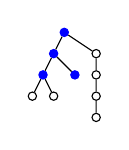
\begin{tikzpicture}[baseline=-0.5ex, scale=0.27]
    \tikzset{every node/.style={draw, circle, inner sep=0.5pt, minimum size=3pt}}
    \node[] (NG) at (-1.80, -3) {};
    \node[] (NH) at (-0.80, -3) {};
    \node[fill=Blue, draw=Blue] (ND) at (-1.30, -2) {};
    \node[fill=Blue, draw=Blue] (NE) at (0.20, -2) {};
    \node[fill=Blue, draw=Blue] (NB) at (-0.80, -1) {};
    \node[] (NJ) at (1.20, -4) {};
    \node[] (NI) at (1.20, -3) {};
    \node[] (NF) at (1.20, -2) {};
    \node[] (NC) at (1.20, -1) {};
    \node[fill=Blue, draw=Blue] (NA) at (-0.30, 0) {};
    \draw (NA) -- (NB);
    \draw (NB) -- (ND);
    \draw (ND) -- (NG);
    \draw (ND) -- (NH);
    \draw (NB) -- (NE);
    \draw (NA) -- (NC);
    \draw (NC) -- (NF);
    \draw (NF) -- (NI);
    \draw (NI) -- (NJ);
  \end{tikzpicture}
}
\newsavebox{\boxshapeb}
\sbox{\boxshapeb}{
  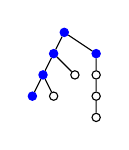
\begin{tikzpicture}[baseline=-0.5ex, scale=0.27]
    \tikzset{every node/.style={draw, circle, inner sep=0.5pt, minimum size=3pt}}
    \node[fill=Blue, draw=Blue] (NG) at (-1.80, -3) {};
    \node[] (NH) at (-0.80, -3) {};
    \node[fill=Blue, draw=Blue] (ND) at (-1.30, -2) {};
    \node[] (NE) at (0.20, -2) {};
    \node[fill=Blue, draw=Blue] (NB) at (-0.80, -1) {};
    \node[] (NJ) at (1.20, -4) {};
    \node[] (NI) at (1.20, -3) {};
    \node[] (NF) at (1.20, -2) {};
    \node[fill=Blue, draw=Blue] (NC) at (1.20, -1) {};
    \node[fill=Blue, draw=Blue] (NA) at (-0.30, 0) {};
    \draw (NA) -- (NB);
    \draw (NB) -- (ND);
    \draw (ND) -- (NG);
    \draw (ND) -- (NH);
    \draw (NB) -- (NE);
    \draw (NA) -- (NC);
    \draw (NC) -- (NF);
    \draw (NF) -- (NI);
    \draw (NI) -- (NJ);
  \end{tikzpicture}
}
\newsavebox{\boxshapec}
\sbox{\boxshapec}{
  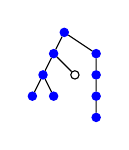
\begin{tikzpicture}[baseline=-0.5ex, scale=0.27]
    \tikzset{every node/.style={draw, circle, inner sep=0.5pt, minimum size=3pt}}
    \node[fill=Blue, draw=Blue] (NG) at (-1.80, -3) {};
    \node[fill=Blue, draw=Blue] (NH) at (-0.80, -3) {};
    \node[fill=Blue, draw=Blue] (ND) at (-1.30, -2) {};
    \node[] (NE) at (0.20, -2) {};
    \node[fill=Blue, draw=Blue] (NB) at (-0.80, -1) {};
    \node[fill=Blue, draw=Blue] (NJ) at (1.20, -4) {};
    \node[fill=Blue, draw=Blue] (NI) at (1.20, -3) {};
    \node[fill=Blue, draw=Blue] (NF) at (1.20, -2) {};
    \node[fill=Blue, draw=Blue] (NC) at (1.20, -1) {};
    \node[fill=Blue, draw=Blue] (NA) at (-0.30, 0) {};
    \draw (NA) -- (NB);
    \draw (NB) -- (ND);
    \draw (ND) -- (NG);
    \draw (ND) -- (NH);
    \draw (NB) -- (NE);
    \draw (NA) -- (NC);
    \draw (NC) -- (NF);
    \draw (NF) -- (NI);
    \draw (NI) -- (NJ);
  \end{tikzpicture}
}
\newsavebox{\boxshaped}
\sbox{\boxshaped}{
  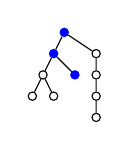
\begin{tikzpicture}[baseline=-0.5ex, scale=0.27]
    \tikzset{every node/.style={draw, circle, inner sep=0.5pt, minimum size=3pt}}
    \node[] (NG) at (-1.80, -3) {};
    \node[] (NH) at (-0.80, -3) {};
    \node[] (ND) at (-1.30, -2) {};
    \node[fill=Blue, draw=Blue] (NE) at (0.20, -2) {};
    \node[fill=Blue, draw=Blue] (NB) at (-0.80, -1) {};
    \node[] (NJ) at (1.20, -4) {};
    \node[] (NI) at (1.20, -3) {};
    \node[] (NF) at (1.20, -2) {};
    \node[] (NC) at (1.20, -1) {};
    \node[fill=Blue, draw=Blue] (NA) at (-0.30, 0) {};
    \draw (NA) -- (NB);
    \draw (NB) -- (ND);
    \draw (ND) -- (NG);
    \draw (ND) -- (NH);
    \draw (NB) -- (NE);
    \draw (NA) -- (NC);
    \draw (NC) -- (NF);
    \draw (NF) -- (NI);
    \draw (NI) -- (NJ);
  \end{tikzpicture}
}
\newsavebox{\boxshapee}
\sbox{\boxshapee}{
  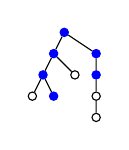
\begin{tikzpicture}[baseline=-0.5ex, scale=0.27]
    \tikzset{every node/.style={draw, circle, inner sep=0.5pt, minimum size=3pt}}
    \node[] (NG) at (-1.80, -3) {};
    \node[fill=Blue, draw=Blue] (NH) at (-0.80, -3) {};
    \node[fill=Blue, draw=Blue] (ND) at (-1.30, -2) {};
    \node[] (NE) at (0.20, -2) {};
    \node[fill=Blue, draw=Blue] (NB) at (-0.80, -1) {};
    \node[] (NJ) at (1.20, -4) {};
    \node[] (NI) at (1.20, -3) {};
    \node[fill=Blue, draw=Blue] (NF) at (1.20, -2) {};
    \node[fill=Blue, draw=Blue] (NC) at (1.20, -1) {};
    \node[fill=Blue, draw=Blue] (NA) at (-0.30, 0) {};
    \draw (NA) -- (NB);
    \draw (NB) -- (ND);
    \draw (ND) -- (NG);
    \draw (ND) -- (NH);
    \draw (NB) -- (NE);
    \draw (NA) -- (NC);
    \draw (NC) -- (NF);
    \draw (NF) -- (NI);
    \draw (NI) -- (NJ);
  \end{tikzpicture}
}
\newsavebox{\boxshapef}
\sbox{\boxshapef}{
  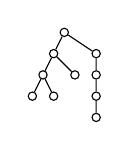
\begin{tikzpicture}[baseline=-0.5ex, scale=0.27]
    \tikzset{every node/.style={draw, circle, inner sep=0.5pt, minimum size=3pt}}
    \node[] (NG) at (-1.80, -3) {};
    \node[] (NH) at (-0.80, -3) {};
    \node[] (ND) at (-1.30, -2) {};
    \node[] (NE) at (0.20, -2) {};
    \node[] (NB) at (-0.80, -1) {};
    \node[] (NJ) at (1.20, -4) {};
    \node[] (NI) at (1.20, -3) {};
    \node[] (NF) at (1.20, -2) {};
    \node[] (NC) at (1.20, -1) {};
    \node[] (NA) at (-0.30, 0) {};
    \draw (NA) -- (NB);
    \draw (NB) -- (ND);
    \draw (ND) -- (NG);
    \draw (ND) -- (NH);
    \draw (NB) -- (NE);
    \draw (NA) -- (NC);
    \draw (NC) -- (NF);
    \draw (NF) -- (NI);
    \draw (NI) -- (NJ);
  \end{tikzpicture}
}
\newsavebox{\boxshapeg}
\sbox{\boxshapeg}{
  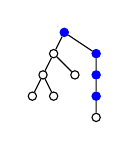
\begin{tikzpicture}[baseline=-0.5ex, scale=0.27]
    \tikzset{every node/.style={draw, circle, inner sep=0.5pt, minimum size=3pt}}
    \node[] (NG) at (-1.80, -3) {};
    \node[] (NH) at (-0.80, -3) {};
    \node[] (ND) at (-1.30, -2) {};
    \node[] (NE) at (0.20, -2) {};
    \node[] (NB) at (-0.80, -1) {};
    \node[] (NJ) at (1.20, -4) {};
    \node[fill=Blue, draw=Blue] (NI) at (1.20, -3) {};
    \node[fill=Blue, draw=Blue] (NF) at (1.20, -2) {};
    \node[fill=Blue, draw=Blue] (NC) at (1.20, -1) {};
    \node[fill=Blue, draw=Blue] (NA) at (-0.30, 0) {};
    \draw (NA) -- (NB);
    \draw (NB) -- (ND);
    \draw (ND) -- (NG);
    \draw (ND) -- (NH);
    \draw (NB) -- (NE);
    \draw (NA) -- (NC);
    \draw (NC) -- (NF);
    \draw (NF) -- (NI);
    \draw (NI) -- (NJ);
  \end{tikzpicture}
}
\newsavebox{\boxshapeh}
\sbox{\boxshapeh}{
  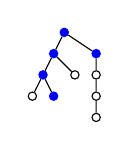
\begin{tikzpicture}[baseline=-0.5ex, scale=0.27]
    \tikzset{every node/.style={draw, circle, inner sep=0.5pt, minimum size=3pt}}
    \node[] (NG) at (-1.80, -3) {};
    \node[fill=Blue, draw=Blue] (NH) at (-0.80, -3) {};
    \node[fill=Blue, draw=Blue] (ND) at (-1.30, -2) {};
    \node[] (NE) at (0.20, -2) {};
    \node[fill=Blue, draw=Blue] (NB) at (-0.80, -1) {};
    \node[] (NJ) at (1.20, -4) {};
    \node[] (NI) at (1.20, -3) {};
    \node[] (NF) at (1.20, -2) {};
    \node[fill=Blue, draw=Blue] (NC) at (1.20, -1) {};
    \node[fill=Blue, draw=Blue] (NA) at (-0.30, 0) {};
    \draw (NA) -- (NB);
    \draw (NB) -- (ND);
    \draw (ND) -- (NG);
    \draw (ND) -- (NH);
    \draw (NB) -- (NE);
    \draw (NA) -- (NC);
    \draw (NC) -- (NF);
    \draw (NF) -- (NI);
    \draw (NI) -- (NJ);
  \end{tikzpicture}
}
\newsavebox{\boxshapei}
\sbox{\boxshapei}{
  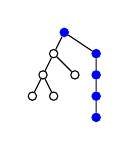
\begin{tikzpicture}[baseline=-0.5ex, scale=0.27]
    \tikzset{every node/.style={draw, circle, inner sep=0.5pt, minimum size=3pt}}
    \node[] (NG) at (-1.80, -3) {};
    \node[] (NH) at (-0.80, -3) {};
    \node[] (ND) at (-1.30, -2) {};
    \node[] (NE) at (0.20, -2) {};
    \node[] (NB) at (-0.80, -1) {};
    \node[fill=Blue, draw=Blue] (NJ) at (1.20, -4) {};
    \node[fill=Blue, draw=Blue] (NI) at (1.20, -3) {};
    \node[fill=Blue, draw=Blue] (NF) at (1.20, -2) {};
    \node[fill=Blue, draw=Blue] (NC) at (1.20, -1) {};
    \node[fill=Blue, draw=Blue] (NA) at (-0.30, 0) {};
    \draw (NA) -- (NB);
    \draw (NB) -- (ND);
    \draw (ND) -- (NG);
    \draw (ND) -- (NH);
    \draw (NB) -- (NE);
    \draw (NA) -- (NC);
    \draw (NC) -- (NF);
    \draw (NF) -- (NI);
    \draw (NI) -- (NJ);
  \end{tikzpicture}
}
\newsavebox{\boxshapej}
\sbox{\boxshapej}{
  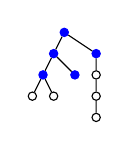
\begin{tikzpicture}[baseline=-0.5ex, scale=0.27]
    \tikzset{every node/.style={draw, circle, inner sep=0.5pt, minimum size=3pt}}
    \node[] (NG) at (-1.80, -3) {};
    \node[] (NH) at (-0.80, -3) {};
    \node[fill=Blue, draw=Blue] (ND) at (-1.30, -2) {};
    \node[fill=Blue, draw=Blue] (NE) at (0.20, -2) {};
    \node[fill=Blue, draw=Blue] (NB) at (-0.80, -1) {};
    \node[] (NJ) at (1.20, -4) {};
    \node[] (NI) at (1.20, -3) {};
    \node[] (NF) at (1.20, -2) {};
    \node[fill=Blue, draw=Blue] (NC) at (1.20, -1) {};
    \node[fill=Blue, draw=Blue] (NA) at (-0.30, 0) {};
    \draw (NA) -- (NB);
    \draw (NB) -- (ND);
    \draw (ND) -- (NG);
    \draw (ND) -- (NH);
    \draw (NB) -- (NE);
    \draw (NA) -- (NC);
    \draw (NC) -- (NF);
    \draw (NF) -- (NI);
    \draw (NI) -- (NJ);
  \end{tikzpicture}
}
\newsavebox{\boxshapek}
\sbox{\boxshapek}{
  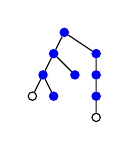
\begin{tikzpicture}[baseline=-0.5ex, scale=0.27]
    \tikzset{every node/.style={draw, circle, inner sep=0.5pt, minimum size=3pt}}
    \node[] (NG) at (-1.80, -3) {};
    \node[fill=Blue, draw=Blue] (NH) at (-0.80, -3) {};
    \node[fill=Blue, draw=Blue] (ND) at (-1.30, -2) {};
    \node[fill=Blue, draw=Blue] (NE) at (0.20, -2) {};
    \node[fill=Blue, draw=Blue] (NB) at (-0.80, -1) {};
    \node[] (NJ) at (1.20, -4) {};
    \node[fill=Blue, draw=Blue] (NI) at (1.20, -3) {};
    \node[fill=Blue, draw=Blue] (NF) at (1.20, -2) {};
    \node[fill=Blue, draw=Blue] (NC) at (1.20, -1) {};
    \node[fill=Blue, draw=Blue] (NA) at (-0.30, 0) {};
    \draw (NA) -- (NB);
    \draw (NB) -- (ND);
    \draw (ND) -- (NG);
    \draw (ND) -- (NH);
    \draw (NB) -- (NE);
    \draw (NA) -- (NC);
    \draw (NC) -- (NF);
    \draw (NF) -- (NI);
    \draw (NI) -- (NJ);
  \end{tikzpicture}
}
\newsavebox{\boxshapel}
\sbox{\boxshapel}{
  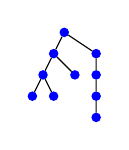
\begin{tikzpicture}[baseline=-0.5ex, scale=0.27]
    \tikzset{every node/.style={draw, circle, inner sep=0.5pt, minimum size=3pt}}
    \node[fill=Blue, draw=Blue] (NG) at (-1.80, -3) {};
    \node[fill=Blue, draw=Blue] (NH) at (-0.80, -3) {};
    \node[fill=Blue, draw=Blue] (ND) at (-1.30, -2) {};
    \node[fill=Blue, draw=Blue] (NE) at (0.20, -2) {};
    \node[fill=Blue, draw=Blue] (NB) at (-0.80, -1) {};
    \node[fill=Blue, draw=Blue] (NJ) at (1.20, -4) {};
    \node[fill=Blue, draw=Blue] (NI) at (1.20, -3) {};
    \node[fill=Blue, draw=Blue] (NF) at (1.20, -2) {};
    \node[fill=Blue, draw=Blue] (NC) at (1.20, -1) {};
    \node[fill=Blue, draw=Blue] (NA) at (-0.30, 0) {};
    \draw (NA) -- (NB);
    \draw (NB) -- (ND);
    \draw (ND) -- (NG);
    \draw (ND) -- (NH);
    \draw (NB) -- (NE);
    \draw (NA) -- (NC);
    \draw (NC) -- (NF);
    \draw (NF) -- (NI);
    \draw (NI) -- (NJ);
  \end{tikzpicture}
}
\newsavebox{\boxshapem}
\sbox{\boxshapem}{
  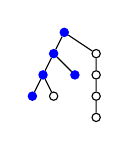
\begin{tikzpicture}[baseline=-0.5ex, scale=0.27]
    \tikzset{every node/.style={draw, circle, inner sep=0.5pt, minimum size=3pt}}
    \node[fill=Blue, draw=Blue] (NG) at (-1.80, -3) {};
    \node[] (NH) at (-0.80, -3) {};
    \node[fill=Blue, draw=Blue] (ND) at (-1.30, -2) {};
    \node[fill=Blue, draw=Blue] (NE) at (0.20, -2) {};
    \node[fill=Blue, draw=Blue] (NB) at (-0.80, -1) {};
    \node[] (NJ) at (1.20, -4) {};
    \node[] (NI) at (1.20, -3) {};
    \node[] (NF) at (1.20, -2) {};
    \node[] (NC) at (1.20, -1) {};
    \node[fill=Blue, draw=Blue] (NA) at (-0.30, 0) {};
    \draw (NA) -- (NB);
    \draw (NB) -- (ND);
    \draw (ND) -- (NG);
    \draw (ND) -- (NH);
    \draw (NB) -- (NE);
    \draw (NA) -- (NC);
    \draw (NC) -- (NF);
    \draw (NF) -- (NI);
    \draw (NI) -- (NJ);
  \end{tikzpicture}
}
\newsavebox{\boxshapen}
\sbox{\boxshapen}{
  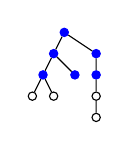
\begin{tikzpicture}[baseline=-0.5ex, scale=0.27]
    \tikzset{every node/.style={draw, circle, inner sep=0.5pt, minimum size=3pt}}
    \node[] (NG) at (-1.80, -3) {};
    \node[] (NH) at (-0.80, -3) {};
    \node[fill=Blue, draw=Blue] (ND) at (-1.30, -2) {};
    \node[fill=Blue, draw=Blue] (NE) at (0.20, -2) {};
    \node[fill=Blue, draw=Blue] (NB) at (-0.80, -1) {};
    \node[] (NJ) at (1.20, -4) {};
    \node[] (NI) at (1.20, -3) {};
    \node[fill=Blue, draw=Blue] (NF) at (1.20, -2) {};
    \node[fill=Blue, draw=Blue] (NC) at (1.20, -1) {};
    \node[fill=Blue, draw=Blue] (NA) at (-0.30, 0) {};
    \draw (NA) -- (NB);
    \draw (NB) -- (ND);
    \draw (ND) -- (NG);
    \draw (ND) -- (NH);
    \draw (NB) -- (NE);
    \draw (NA) -- (NC);
    \draw (NC) -- (NF);
    \draw (NF) -- (NI);
    \draw (NI) -- (NJ);
  \end{tikzpicture}
}
\newsavebox{\boxshapeo}
\sbox{\boxshapeo}{
  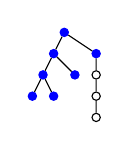
\begin{tikzpicture}[baseline=-0.5ex, scale=0.27]
    \tikzset{every node/.style={draw, circle, inner sep=0.5pt, minimum size=3pt}}
    \node[fill=Blue, draw=Blue] (NG) at (-1.80, -3) {};
    \node[fill=Blue, draw=Blue] (NH) at (-0.80, -3) {};
    \node[fill=Blue, draw=Blue] (ND) at (-1.30, -2) {};
    \node[fill=Blue, draw=Blue] (NE) at (0.20, -2) {};
    \node[fill=Blue, draw=Blue] (NB) at (-0.80, -1) {};
    \node[] (NJ) at (1.20, -4) {};
    \node[] (NI) at (1.20, -3) {};
    \node[] (NF) at (1.20, -2) {};
    \node[fill=Blue, draw=Blue] (NC) at (1.20, -1) {};
    \node[fill=Blue, draw=Blue] (NA) at (-0.30, 0) {};
    \draw (NA) -- (NB);
    \draw (NB) -- (ND);
    \draw (ND) -- (NG);
    \draw (ND) -- (NH);
    \draw (NB) -- (NE);
    \draw (NA) -- (NC);
    \draw (NC) -- (NF);
    \draw (NF) -- (NI);
    \draw (NI) -- (NJ);
  \end{tikzpicture}
}
\newsavebox{\boxshapep}
\sbox{\boxshapep}{
  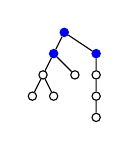
\begin{tikzpicture}[baseline=-0.5ex, scale=0.27]
    \tikzset{every node/.style={draw, circle, inner sep=0.5pt, minimum size=3pt}}
    \node[] (NG) at (-1.80, -3) {};
    \node[] (NH) at (-0.80, -3) {};
    \node[] (ND) at (-1.30, -2) {};
    \node[] (NE) at (0.20, -2) {};
    \node[fill=Blue, draw=Blue] (NB) at (-0.80, -1) {};
    \node[] (NJ) at (1.20, -4) {};
    \node[] (NI) at (1.20, -3) {};
    \node[] (NF) at (1.20, -2) {};
    \node[fill=Blue, draw=Blue] (NC) at (1.20, -1) {};
    \node[fill=Blue, draw=Blue] (NA) at (-0.30, 0) {};
    \draw (NA) -- (NB);
    \draw (NB) -- (ND);
    \draw (ND) -- (NG);
    \draw (ND) -- (NH);
    \draw (NB) -- (NE);
    \draw (NA) -- (NC);
    \draw (NC) -- (NF);
    \draw (NF) -- (NI);
    \draw (NI) -- (NJ);
  \end{tikzpicture}
}
\newsavebox{\boxshapeq}
\sbox{\boxshapeq}{
  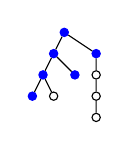
\begin{tikzpicture}[baseline=-0.5ex, scale=0.27]
    \tikzset{every node/.style={draw, circle, inner sep=0.5pt, minimum size=3pt}}
    \node[fill=Blue, draw=Blue] (NG) at (-1.80, -3) {};
    \node[] (NH) at (-0.80, -3) {};
    \node[fill=Blue, draw=Blue] (ND) at (-1.30, -2) {};
    \node[fill=Blue, draw=Blue] (NE) at (0.20, -2) {};
    \node[fill=Blue, draw=Blue] (NB) at (-0.80, -1) {};
    \node[] (NJ) at (1.20, -4) {};
    \node[] (NI) at (1.20, -3) {};
    \node[] (NF) at (1.20, -2) {};
    \node[fill=Blue, draw=Blue] (NC) at (1.20, -1) {};
    \node[fill=Blue, draw=Blue] (NA) at (-0.30, 0) {};
    \draw (NA) -- (NB);
    \draw (NB) -- (ND);
    \draw (ND) -- (NG);
    \draw (ND) -- (NH);
    \draw (NB) -- (NE);
    \draw (NA) -- (NC);
    \draw (NC) -- (NF);
    \draw (NF) -- (NI);
    \draw (NI) -- (NJ);
  \end{tikzpicture}
}
\newsavebox{\boxshaper}
\sbox{\boxshaper}{
  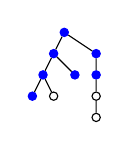
\begin{tikzpicture}[baseline=-0.5ex, scale=0.27]
    \tikzset{every node/.style={draw, circle, inner sep=0.5pt, minimum size=3pt}}
    \node[fill=Blue, draw=Blue] (NG) at (-1.80, -3) {};
    \node[] (NH) at (-0.80, -3) {};
    \node[fill=Blue, draw=Blue] (ND) at (-1.30, -2) {};
    \node[fill=Blue, draw=Blue] (NE) at (0.20, -2) {};
    \node[fill=Blue, draw=Blue] (NB) at (-0.80, -1) {};
    \node[] (NJ) at (1.20, -4) {};
    \node[] (NI) at (1.20, -3) {};
    \node[fill=Blue, draw=Blue] (NF) at (1.20, -2) {};
    \node[fill=Blue, draw=Blue] (NC) at (1.20, -1) {};
    \node[fill=Blue, draw=Blue] (NA) at (-0.30, 0) {};
    \draw (NA) -- (NB);
    \draw (NB) -- (ND);
    \draw (ND) -- (NG);
    \draw (ND) -- (NH);
    \draw (NB) -- (NE);
    \draw (NA) -- (NC);
    \draw (NC) -- (NF);
    \draw (NF) -- (NI);
    \draw (NI) -- (NJ);
  \end{tikzpicture}
}
\newsavebox{\boxshapes}
\sbox{\boxshapes}{
  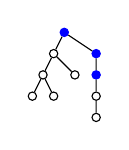
\begin{tikzpicture}[baseline=-0.5ex, scale=0.27]
    \tikzset{every node/.style={draw, circle, inner sep=0.5pt, minimum size=3pt}}
    \node[] (NG) at (-1.80, -3) {};
    \node[] (NH) at (-0.80, -3) {};
    \node[] (ND) at (-1.30, -2) {};
    \node[] (NE) at (0.20, -2) {};
    \node[] (NB) at (-0.80, -1) {};
    \node[] (NJ) at (1.20, -4) {};
    \node[] (NI) at (1.20, -3) {};
    \node[fill=Blue, draw=Blue] (NF) at (1.20, -2) {};
    \node[fill=Blue, draw=Blue] (NC) at (1.20, -1) {};
    \node[fill=Blue, draw=Blue] (NA) at (-0.30, 0) {};
    \draw (NA) -- (NB);
    \draw (NB) -- (ND);
    \draw (ND) -- (NG);
    \draw (ND) -- (NH);
    \draw (NB) -- (NE);
    \draw (NA) -- (NC);
    \draw (NC) -- (NF);
    \draw (NF) -- (NI);
    \draw (NI) -- (NJ);
  \end{tikzpicture}
}
\newsavebox{\boxshapet}
\sbox{\boxshapet}{
  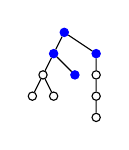
\begin{tikzpicture}[baseline=-0.5ex, scale=0.27]
    \tikzset{every node/.style={draw, circle, inner sep=0.5pt, minimum size=3pt}}
    \node[] (NG) at (-1.80, -3) {};
    \node[] (NH) at (-0.80, -3) {};
    \node[] (ND) at (-1.30, -2) {};
    \node[fill=Blue, draw=Blue] (NE) at (0.20, -2) {};
    \node[fill=Blue, draw=Blue] (NB) at (-0.80, -1) {};
    \node[] (NJ) at (1.20, -4) {};
    \node[] (NI) at (1.20, -3) {};
    \node[] (NF) at (1.20, -2) {};
    \node[fill=Blue, draw=Blue] (NC) at (1.20, -1) {};
    \node[fill=Blue, draw=Blue] (NA) at (-0.30, 0) {};
    \draw (NA) -- (NB);
    \draw (NB) -- (ND);
    \draw (ND) -- (NG);
    \draw (ND) -- (NH);
    \draw (NB) -- (NE);
    \draw (NA) -- (NC);
    \draw (NC) -- (NF);
    \draw (NF) -- (NI);
    \draw (NI) -- (NJ);
  \end{tikzpicture}
}
\newsavebox{\boxshapeu}
\sbox{\boxshapeu}{
  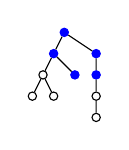
\begin{tikzpicture}[baseline=-0.5ex, scale=0.27]
    \tikzset{every node/.style={draw, circle, inner sep=0.5pt, minimum size=3pt}}
    \node[] (NG) at (-1.80, -3) {};
    \node[] (NH) at (-0.80, -3) {};
    \node[] (ND) at (-1.30, -2) {};
    \node[fill=Blue, draw=Blue] (NE) at (0.20, -2) {};
    \node[fill=Blue, draw=Blue] (NB) at (-0.80, -1) {};
    \node[] (NJ) at (1.20, -4) {};
    \node[] (NI) at (1.20, -3) {};
    \node[fill=Blue, draw=Blue] (NF) at (1.20, -2) {};
    \node[fill=Blue, draw=Blue] (NC) at (1.20, -1) {};
    \node[fill=Blue, draw=Blue] (NA) at (-0.30, 0) {};
    \draw (NA) -- (NB);
    \draw (NB) -- (ND);
    \draw (ND) -- (NG);
    \draw (ND) -- (NH);
    \draw (NB) -- (NE);
    \draw (NA) -- (NC);
    \draw (NC) -- (NF);
    \draw (NF) -- (NI);
    \draw (NI) -- (NJ);
  \end{tikzpicture}
}
\newsavebox{\boxshapev}
\sbox{\boxshapev}{
  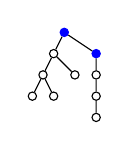
\begin{tikzpicture}[baseline=-0.5ex, scale=0.27]
    \tikzset{every node/.style={draw, circle, inner sep=0.5pt, minimum size=3pt}}
    \node[] (NG) at (-1.80, -3) {};
    \node[] (NH) at (-0.80, -3) {};
    \node[] (ND) at (-1.30, -2) {};
    \node[] (NE) at (0.20, -2) {};
    \node[] (NB) at (-0.80, -1) {};
    \node[] (NJ) at (1.20, -4) {};
    \node[] (NI) at (1.20, -3) {};
    \node[] (NF) at (1.20, -2) {};
    \node[fill=Blue, draw=Blue] (NC) at (1.20, -1) {};
    \node[fill=Blue, draw=Blue] (NA) at (-0.30, 0) {};
    \draw (NA) -- (NB);
    \draw (NB) -- (ND);
    \draw (ND) -- (NG);
    \draw (ND) -- (NH);
    \draw (NB) -- (NE);
    \draw (NA) -- (NC);
    \draw (NC) -- (NF);
    \draw (NF) -- (NI);
    \draw (NI) -- (NJ);
  \end{tikzpicture}
}
\newsavebox{\boxshapew}
\sbox{\boxshapew}{
  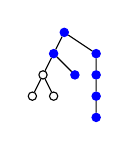
\begin{tikzpicture}[baseline=-0.5ex, scale=0.27]
    \tikzset{every node/.style={draw, circle, inner sep=0.5pt, minimum size=3pt}}
    \node[] (NG) at (-1.80, -3) {};
    \node[] (NH) at (-0.80, -3) {};
    \node[] (ND) at (-1.30, -2) {};
    \node[fill=Blue, draw=Blue] (NE) at (0.20, -2) {};
    \node[fill=Blue, draw=Blue] (NB) at (-0.80, -1) {};
    \node[fill=Blue, draw=Blue] (NJ) at (1.20, -4) {};
    \node[fill=Blue, draw=Blue] (NI) at (1.20, -3) {};
    \node[fill=Blue, draw=Blue] (NF) at (1.20, -2) {};
    \node[fill=Blue, draw=Blue] (NC) at (1.20, -1) {};
    \node[fill=Blue, draw=Blue] (NA) at (-0.30, 0) {};
    \draw (NA) -- (NB);
    \draw (NB) -- (ND);
    \draw (ND) -- (NG);
    \draw (ND) -- (NH);
    \draw (NB) -- (NE);
    \draw (NA) -- (NC);
    \draw (NC) -- (NF);
    \draw (NF) -- (NI);
    \draw (NI) -- (NJ);
  \end{tikzpicture}
}
\newsavebox{\boxshapex}
\sbox{\boxshapex}{
  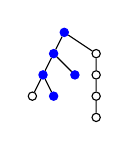
\begin{tikzpicture}[baseline=-0.5ex, scale=0.27]
    \tikzset{every node/.style={draw, circle, inner sep=0.5pt, minimum size=3pt}}
    \node[] (NG) at (-1.80, -3) {};
    \node[fill=Blue, draw=Blue] (NH) at (-0.80, -3) {};
    \node[fill=Blue, draw=Blue] (ND) at (-1.30, -2) {};
    \node[fill=Blue, draw=Blue] (NE) at (0.20, -2) {};
    \node[fill=Blue, draw=Blue] (NB) at (-0.80, -1) {};
    \node[] (NJ) at (1.20, -4) {};
    \node[] (NI) at (1.20, -3) {};
    \node[] (NF) at (1.20, -2) {};
    \node[] (NC) at (1.20, -1) {};
    \node[fill=Blue, draw=Blue] (NA) at (-0.30, 0) {};
    \draw (NA) -- (NB);
    \draw (NB) -- (ND);
    \draw (ND) -- (NG);
    \draw (ND) -- (NH);
    \draw (NB) -- (NE);
    \draw (NA) -- (NC);
    \draw (NC) -- (NF);
    \draw (NF) -- (NI);
    \draw (NI) -- (NJ);
  \end{tikzpicture}
}
\newsavebox{\boxshapey}
\sbox{\boxshapey}{
  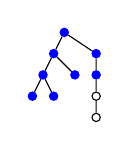
\begin{tikzpicture}[baseline=-0.5ex, scale=0.27]
    \tikzset{every node/.style={draw, circle, inner sep=0.5pt, minimum size=3pt}}
    \node[fill=Blue, draw=Blue] (NG) at (-1.80, -3) {};
    \node[fill=Blue, draw=Blue] (NH) at (-0.80, -3) {};
    \node[fill=Blue, draw=Blue] (ND) at (-1.30, -2) {};
    \node[fill=Blue, draw=Blue] (NE) at (0.20, -2) {};
    \node[fill=Blue, draw=Blue] (NB) at (-0.80, -1) {};
    \node[] (NJ) at (1.20, -4) {};
    \node[] (NI) at (1.20, -3) {};
    \node[fill=Blue, draw=Blue] (NF) at (1.20, -2) {};
    \node[fill=Blue, draw=Blue] (NC) at (1.20, -1) {};
    \node[fill=Blue, draw=Blue] (NA) at (-0.30, 0) {};
    \draw (NA) -- (NB);
    \draw (NB) -- (ND);
    \draw (ND) -- (NG);
    \draw (ND) -- (NH);
    \draw (NB) -- (NE);
    \draw (NA) -- (NC);
    \draw (NC) -- (NF);
    \draw (NF) -- (NI);
    \draw (NI) -- (NJ);
  \end{tikzpicture}
}
\newsavebox{\boxshapez}
\sbox{\boxshapez}{
  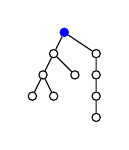
\begin{tikzpicture}[baseline=-0.5ex, scale=0.27]
    \tikzset{every node/.style={draw, circle, inner sep=0.5pt, minimum size=3pt}}
    \node[] (NG) at (-1.80, -3) {};
    \node[] (NH) at (-0.80, -3) {};
    \node[] (ND) at (-1.30, -2) {};
    \node[] (NE) at (0.20, -2) {};
    \node[] (NB) at (-0.80, -1) {};
    \node[] (NJ) at (1.20, -4) {};
    \node[] (NI) at (1.20, -3) {};
    \node[] (NF) at (1.20, -2) {};
    \node[] (NC) at (1.20, -1) {};
    \node[fill=Blue, draw=Blue] (NA) at (-0.30, 0) {};
    \draw (NA) -- (NB);
    \draw (NB) -- (ND);
    \draw (ND) -- (NG);
    \draw (ND) -- (NH);
    \draw (NB) -- (NE);
    \draw (NA) -- (NC);
    \draw (NC) -- (NF);
    \draw (NF) -- (NI);
    \draw (NI) -- (NJ);
  \end{tikzpicture}
}
\newsavebox{\boxshapeaa}
\sbox{\boxshapeaa}{
  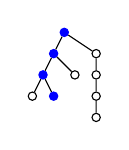
\begin{tikzpicture}[baseline=-0.5ex, scale=0.27]
    \tikzset{every node/.style={draw, circle, inner sep=0.5pt, minimum size=3pt}}
    \node[] (NG) at (-1.80, -3) {};
    \node[fill=Blue, draw=Blue] (NH) at (-0.80, -3) {};
    \node[fill=Blue, draw=Blue] (ND) at (-1.30, -2) {};
    \node[] (NE) at (0.20, -2) {};
    \node[fill=Blue, draw=Blue] (NB) at (-0.80, -1) {};
    \node[] (NJ) at (1.20, -4) {};
    \node[] (NI) at (1.20, -3) {};
    \node[] (NF) at (1.20, -2) {};
    \node[] (NC) at (1.20, -1) {};
    \node[fill=Blue, draw=Blue] (NA) at (-0.30, 0) {};
    \draw (NA) -- (NB);
    \draw (NB) -- (ND);
    \draw (ND) -- (NG);
    \draw (ND) -- (NH);
    \draw (NB) -- (NE);
    \draw (NA) -- (NC);
    \draw (NC) -- (NF);
    \draw (NF) -- (NI);
    \draw (NI) -- (NJ);
  \end{tikzpicture}
}
\newsavebox{\boxshapeab}
\sbox{\boxshapeab}{
  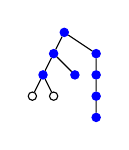
\begin{tikzpicture}[baseline=-0.5ex, scale=0.27]
    \tikzset{every node/.style={draw, circle, inner sep=0.5pt, minimum size=3pt}}
    \node[] (NG) at (-1.80, -3) {};
    \node[] (NH) at (-0.80, -3) {};
    \node[fill=Blue, draw=Blue] (ND) at (-1.30, -2) {};
    \node[fill=Blue, draw=Blue] (NE) at (0.20, -2) {};
    \node[fill=Blue, draw=Blue] (NB) at (-0.80, -1) {};
    \node[fill=Blue, draw=Blue] (NJ) at (1.20, -4) {};
    \node[fill=Blue, draw=Blue] (NI) at (1.20, -3) {};
    \node[fill=Blue, draw=Blue] (NF) at (1.20, -2) {};
    \node[fill=Blue, draw=Blue] (NC) at (1.20, -1) {};
    \node[fill=Blue, draw=Blue] (NA) at (-0.30, 0) {};
    \draw (NA) -- (NB);
    \draw (NB) -- (ND);
    \draw (ND) -- (NG);
    \draw (ND) -- (NH);
    \draw (NB) -- (NE);
    \draw (NA) -- (NC);
    \draw (NC) -- (NF);
    \draw (NF) -- (NI);
    \draw (NI) -- (NJ);
  \end{tikzpicture}
}
\newsavebox{\boxshapeac}
\sbox{\boxshapeac}{
  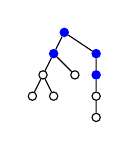
\begin{tikzpicture}[baseline=-0.5ex, scale=0.27]
    \tikzset{every node/.style={draw, circle, inner sep=0.5pt, minimum size=3pt}}
    \node[] (NG) at (-1.80, -3) {};
    \node[] (NH) at (-0.80, -3) {};
    \node[] (ND) at (-1.30, -2) {};
    \node[] (NE) at (0.20, -2) {};
    \node[fill=Blue, draw=Blue] (NB) at (-0.80, -1) {};
    \node[] (NJ) at (1.20, -4) {};
    \node[] (NI) at (1.20, -3) {};
    \node[fill=Blue, draw=Blue] (NF) at (1.20, -2) {};
    \node[fill=Blue, draw=Blue] (NC) at (1.20, -1) {};
    \node[fill=Blue, draw=Blue] (NA) at (-0.30, 0) {};
    \draw (NA) -- (NB);
    \draw (NB) -- (ND);
    \draw (ND) -- (NG);
    \draw (ND) -- (NH);
    \draw (NB) -- (NE);
    \draw (NA) -- (NC);
    \draw (NC) -- (NF);
    \draw (NF) -- (NI);
    \draw (NI) -- (NJ);
  \end{tikzpicture}
}
\newsavebox{\boxshapead}
\sbox{\boxshapead}{
  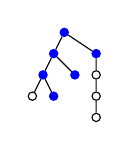
\begin{tikzpicture}[baseline=-0.5ex, scale=0.27]
    \tikzset{every node/.style={draw, circle, inner sep=0.5pt, minimum size=3pt}}
    \node[] (NG) at (-1.80, -3) {};
    \node[fill=Blue, draw=Blue] (NH) at (-0.80, -3) {};
    \node[fill=Blue, draw=Blue] (ND) at (-1.30, -2) {};
    \node[fill=Blue, draw=Blue] (NE) at (0.20, -2) {};
    \node[fill=Blue, draw=Blue] (NB) at (-0.80, -1) {};
    \node[] (NJ) at (1.20, -4) {};
    \node[] (NI) at (1.20, -3) {};
    \node[] (NF) at (1.20, -2) {};
    \node[fill=Blue, draw=Blue] (NC) at (1.20, -1) {};
    \node[fill=Blue, draw=Blue] (NA) at (-0.30, 0) {};
    \draw (NA) -- (NB);
    \draw (NB) -- (ND);
    \draw (ND) -- (NG);
    \draw (ND) -- (NH);
    \draw (NB) -- (NE);
    \draw (NA) -- (NC);
    \draw (NC) -- (NF);
    \draw (NF) -- (NI);
    \draw (NI) -- (NJ);
  \end{tikzpicture}
}
\newsavebox{\boxshapeae}
\sbox{\boxshapeae}{
  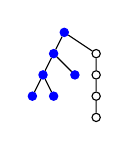
\begin{tikzpicture}[baseline=-0.5ex, scale=0.27]
    \tikzset{every node/.style={draw, circle, inner sep=0.5pt, minimum size=3pt}}
    \node[fill=Blue, draw=Blue] (NG) at (-1.80, -3) {};
    \node[fill=Blue, draw=Blue] (NH) at (-0.80, -3) {};
    \node[fill=Blue, draw=Blue] (ND) at (-1.30, -2) {};
    \node[fill=Blue, draw=Blue] (NE) at (0.20, -2) {};
    \node[fill=Blue, draw=Blue] (NB) at (-0.80, -1) {};
    \node[] (NJ) at (1.20, -4) {};
    \node[] (NI) at (1.20, -3) {};
    \node[] (NF) at (1.20, -2) {};
    \node[] (NC) at (1.20, -1) {};
    \node[fill=Blue, draw=Blue] (NA) at (-0.30, 0) {};
    \draw (NA) -- (NB);
    \draw (NB) -- (ND);
    \draw (ND) -- (NG);
    \draw (ND) -- (NH);
    \draw (NB) -- (NE);
    \draw (NA) -- (NC);
    \draw (NC) -- (NF);
    \draw (NF) -- (NI);
    \draw (NI) -- (NJ);
  \end{tikzpicture}
}
\newsavebox{\boxshapeaf}
\sbox{\boxshapeaf}{
  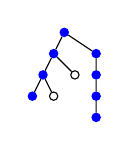
\begin{tikzpicture}[baseline=-0.5ex, scale=0.27]
    \tikzset{every node/.style={draw, circle, inner sep=0.5pt, minimum size=3pt}}
    \node[fill=Blue, draw=Blue] (NG) at (-1.80, -3) {};
    \node[] (NH) at (-0.80, -3) {};
    \node[fill=Blue, draw=Blue] (ND) at (-1.30, -2) {};
    \node[] (NE) at (0.20, -2) {};
    \node[fill=Blue, draw=Blue] (NB) at (-0.80, -1) {};
    \node[fill=Blue, draw=Blue] (NJ) at (1.20, -4) {};
    \node[fill=Blue, draw=Blue] (NI) at (1.20, -3) {};
    \node[fill=Blue, draw=Blue] (NF) at (1.20, -2) {};
    \node[fill=Blue, draw=Blue] (NC) at (1.20, -1) {};
    \node[fill=Blue, draw=Blue] (NA) at (-0.30, 0) {};
    \draw (NA) -- (NB);
    \draw (NB) -- (ND);
    \draw (ND) -- (NG);
    \draw (ND) -- (NH);
    \draw (NB) -- (NE);
    \draw (NA) -- (NC);
    \draw (NC) -- (NF);
    \draw (NF) -- (NI);
    \draw (NI) -- (NJ);
  \end{tikzpicture}
}
\newsavebox{\boxshapeag}
\sbox{\boxshapeag}{
  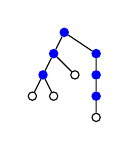
\begin{tikzpicture}[baseline=-0.5ex, scale=0.27]
    \tikzset{every node/.style={draw, circle, inner sep=0.5pt, minimum size=3pt}}
    \node[] (NG) at (-1.80, -3) {};
    \node[] (NH) at (-0.80, -3) {};
    \node[fill=Blue, draw=Blue] (ND) at (-1.30, -2) {};
    \node[] (NE) at (0.20, -2) {};
    \node[fill=Blue, draw=Blue] (NB) at (-0.80, -1) {};
    \node[] (NJ) at (1.20, -4) {};
    \node[fill=Blue, draw=Blue] (NI) at (1.20, -3) {};
    \node[fill=Blue, draw=Blue] (NF) at (1.20, -2) {};
    \node[fill=Blue, draw=Blue] (NC) at (1.20, -1) {};
    \node[fill=Blue, draw=Blue] (NA) at (-0.30, 0) {};
    \draw (NA) -- (NB);
    \draw (NB) -- (ND);
    \draw (ND) -- (NG);
    \draw (ND) -- (NH);
    \draw (NB) -- (NE);
    \draw (NA) -- (NC);
    \draw (NC) -- (NF);
    \draw (NF) -- (NI);
    \draw (NI) -- (NJ);
  \end{tikzpicture}
}
\newsavebox{\boxshapeah}
\sbox{\boxshapeah}{
  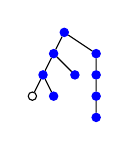
\begin{tikzpicture}[baseline=-0.5ex, scale=0.27]
    \tikzset{every node/.style={draw, circle, inner sep=0.5pt, minimum size=3pt}}
    \node[] (NG) at (-1.80, -3) {};
    \node[fill=Blue, draw=Blue] (NH) at (-0.80, -3) {};
    \node[fill=Blue, draw=Blue] (ND) at (-1.30, -2) {};
    \node[fill=Blue, draw=Blue] (NE) at (0.20, -2) {};
    \node[fill=Blue, draw=Blue] (NB) at (-0.80, -1) {};
    \node[fill=Blue, draw=Blue] (NJ) at (1.20, -4) {};
    \node[fill=Blue, draw=Blue] (NI) at (1.20, -3) {};
    \node[fill=Blue, draw=Blue] (NF) at (1.20, -2) {};
    \node[fill=Blue, draw=Blue] (NC) at (1.20, -1) {};
    \node[fill=Blue, draw=Blue] (NA) at (-0.30, 0) {};
    \draw (NA) -- (NB);
    \draw (NB) -- (ND);
    \draw (ND) -- (NG);
    \draw (ND) -- (NH);
    \draw (NB) -- (NE);
    \draw (NA) -- (NC);
    \draw (NC) -- (NF);
    \draw (NF) -- (NI);
    \draw (NI) -- (NJ);
  \end{tikzpicture}
}
\newsavebox{\boxshapeai}
\sbox{\boxshapeai}{
  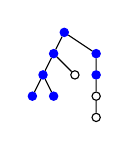
\begin{tikzpicture}[baseline=-0.5ex, scale=0.27]
    \tikzset{every node/.style={draw, circle, inner sep=0.5pt, minimum size=3pt}}
    \node[fill=Blue, draw=Blue] (NG) at (-1.80, -3) {};
    \node[fill=Blue, draw=Blue] (NH) at (-0.80, -3) {};
    \node[fill=Blue, draw=Blue] (ND) at (-1.30, -2) {};
    \node[] (NE) at (0.20, -2) {};
    \node[fill=Blue, draw=Blue] (NB) at (-0.80, -1) {};
    \node[] (NJ) at (1.20, -4) {};
    \node[] (NI) at (1.20, -3) {};
    \node[fill=Blue, draw=Blue] (NF) at (1.20, -2) {};
    \node[fill=Blue, draw=Blue] (NC) at (1.20, -1) {};
    \node[fill=Blue, draw=Blue] (NA) at (-0.30, 0) {};
    \draw (NA) -- (NB);
    \draw (NB) -- (ND);
    \draw (ND) -- (NG);
    \draw (ND) -- (NH);
    \draw (NB) -- (NE);
    \draw (NA) -- (NC);
    \draw (NC) -- (NF);
    \draw (NF) -- (NI);
    \draw (NI) -- (NJ);
  \end{tikzpicture}
}
\newsavebox{\boxshapeaj}
\sbox{\boxshapeaj}{
  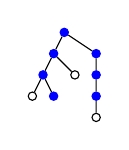
\begin{tikzpicture}[baseline=-0.5ex, scale=0.27]
    \tikzset{every node/.style={draw, circle, inner sep=0.5pt, minimum size=3pt}}
    \node[] (NG) at (-1.80, -3) {};
    \node[fill=Blue, draw=Blue] (NH) at (-0.80, -3) {};
    \node[fill=Blue, draw=Blue] (ND) at (-1.30, -2) {};
    \node[] (NE) at (0.20, -2) {};
    \node[fill=Blue, draw=Blue] (NB) at (-0.80, -1) {};
    \node[] (NJ) at (1.20, -4) {};
    \node[fill=Blue, draw=Blue] (NI) at (1.20, -3) {};
    \node[fill=Blue, draw=Blue] (NF) at (1.20, -2) {};
    \node[fill=Blue, draw=Blue] (NC) at (1.20, -1) {};
    \node[fill=Blue, draw=Blue] (NA) at (-0.30, 0) {};
    \draw (NA) -- (NB);
    \draw (NB) -- (ND);
    \draw (ND) -- (NG);
    \draw (ND) -- (NH);
    \draw (NB) -- (NE);
    \draw (NA) -- (NC);
    \draw (NC) -- (NF);
    \draw (NF) -- (NI);
    \draw (NI) -- (NJ);
  \end{tikzpicture}
}
\newsavebox{\boxshapeak}
\sbox{\boxshapeak}{
  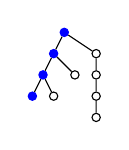
\begin{tikzpicture}[baseline=-0.5ex, scale=0.27]
    \tikzset{every node/.style={draw, circle, inner sep=0.5pt, minimum size=3pt}}
    \node[fill=Blue, draw=Blue] (NG) at (-1.80, -3) {};
    \node[] (NH) at (-0.80, -3) {};
    \node[fill=Blue, draw=Blue] (ND) at (-1.30, -2) {};
    \node[] (NE) at (0.20, -2) {};
    \node[fill=Blue, draw=Blue] (NB) at (-0.80, -1) {};
    \node[] (NJ) at (1.20, -4) {};
    \node[] (NI) at (1.20, -3) {};
    \node[] (NF) at (1.20, -2) {};
    \node[] (NC) at (1.20, -1) {};
    \node[fill=Blue, draw=Blue] (NA) at (-0.30, 0) {};
    \draw (NA) -- (NB);
    \draw (NB) -- (ND);
    \draw (ND) -- (NG);
    \draw (ND) -- (NH);
    \draw (NB) -- (NE);
    \draw (NA) -- (NC);
    \draw (NC) -- (NF);
    \draw (NF) -- (NI);
    \draw (NI) -- (NJ);
  \end{tikzpicture}
}
\newsavebox{\boxshapeal}
\sbox{\boxshapeal}{
  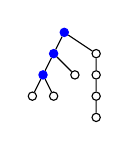
\begin{tikzpicture}[baseline=-0.5ex, scale=0.27]
    \tikzset{every node/.style={draw, circle, inner sep=0.5pt, minimum size=3pt}}
    \node[] (NG) at (-1.80, -3) {};
    \node[] (NH) at (-0.80, -3) {};
    \node[fill=Blue, draw=Blue] (ND) at (-1.30, -2) {};
    \node[] (NE) at (0.20, -2) {};
    \node[fill=Blue, draw=Blue] (NB) at (-0.80, -1) {};
    \node[] (NJ) at (1.20, -4) {};
    \node[] (NI) at (1.20, -3) {};
    \node[] (NF) at (1.20, -2) {};
    \node[] (NC) at (1.20, -1) {};
    \node[fill=Blue, draw=Blue] (NA) at (-0.30, 0) {};
    \draw (NA) -- (NB);
    \draw (NB) -- (ND);
    \draw (ND) -- (NG);
    \draw (ND) -- (NH);
    \draw (NB) -- (NE);
    \draw (NA) -- (NC);
    \draw (NC) -- (NF);
    \draw (NF) -- (NI);
    \draw (NI) -- (NJ);
  \end{tikzpicture}
}
\newsavebox{\boxshapeam}
\sbox{\boxshapeam}{
  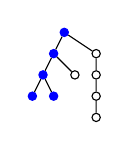
\begin{tikzpicture}[baseline=-0.5ex, scale=0.27]
    \tikzset{every node/.style={draw, circle, inner sep=0.5pt, minimum size=3pt}}
    \node[fill=Blue, draw=Blue] (NG) at (-1.80, -3) {};
    \node[fill=Blue, draw=Blue] (NH) at (-0.80, -3) {};
    \node[fill=Blue, draw=Blue] (ND) at (-1.30, -2) {};
    \node[] (NE) at (0.20, -2) {};
    \node[fill=Blue, draw=Blue] (NB) at (-0.80, -1) {};
    \node[] (NJ) at (1.20, -4) {};
    \node[] (NI) at (1.20, -3) {};
    \node[] (NF) at (1.20, -2) {};
    \node[] (NC) at (1.20, -1) {};
    \node[fill=Blue, draw=Blue] (NA) at (-0.30, 0) {};
    \draw (NA) -- (NB);
    \draw (NB) -- (ND);
    \draw (ND) -- (NG);
    \draw (ND) -- (NH);
    \draw (NB) -- (NE);
    \draw (NA) -- (NC);
    \draw (NC) -- (NF);
    \draw (NF) -- (NI);
    \draw (NI) -- (NJ);
  \end{tikzpicture}
}
\newsavebox{\boxshapean}
\sbox{\boxshapean}{
  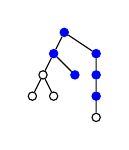
\begin{tikzpicture}[baseline=-0.5ex, scale=0.27]
    \tikzset{every node/.style={draw, circle, inner sep=0.5pt, minimum size=3pt}}
    \node[] (NG) at (-1.80, -3) {};
    \node[] (NH) at (-0.80, -3) {};
    \node[] (ND) at (-1.30, -2) {};
    \node[fill=Blue, draw=Blue] (NE) at (0.20, -2) {};
    \node[fill=Blue, draw=Blue] (NB) at (-0.80, -1) {};
    \node[] (NJ) at (1.20, -4) {};
    \node[fill=Blue, draw=Blue] (NI) at (1.20, -3) {};
    \node[fill=Blue, draw=Blue] (NF) at (1.20, -2) {};
    \node[fill=Blue, draw=Blue] (NC) at (1.20, -1) {};
    \node[fill=Blue, draw=Blue] (NA) at (-0.30, 0) {};
    \draw (NA) -- (NB);
    \draw (NB) -- (ND);
    \draw (ND) -- (NG);
    \draw (ND) -- (NH);
    \draw (NB) -- (NE);
    \draw (NA) -- (NC);
    \draw (NC) -- (NF);
    \draw (NF) -- (NI);
    \draw (NI) -- (NJ);
  \end{tikzpicture}
}
\newsavebox{\boxshapeao}
\sbox{\boxshapeao}{
  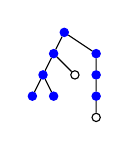
\begin{tikzpicture}[baseline=-0.5ex, scale=0.27]
    \tikzset{every node/.style={draw, circle, inner sep=0.5pt, minimum size=3pt}}
    \node[fill=Blue, draw=Blue] (NG) at (-1.80, -3) {};
    \node[fill=Blue, draw=Blue] (NH) at (-0.80, -3) {};
    \node[fill=Blue, draw=Blue] (ND) at (-1.30, -2) {};
    \node[] (NE) at (0.20, -2) {};
    \node[fill=Blue, draw=Blue] (NB) at (-0.80, -1) {};
    \node[] (NJ) at (1.20, -4) {};
    \node[fill=Blue, draw=Blue] (NI) at (1.20, -3) {};
    \node[fill=Blue, draw=Blue] (NF) at (1.20, -2) {};
    \node[fill=Blue, draw=Blue] (NC) at (1.20, -1) {};
    \node[fill=Blue, draw=Blue] (NA) at (-0.30, 0) {};
    \draw (NA) -- (NB);
    \draw (NB) -- (ND);
    \draw (ND) -- (NG);
    \draw (ND) -- (NH);
    \draw (NB) -- (NE);
    \draw (NA) -- (NC);
    \draw (NC) -- (NF);
    \draw (NF) -- (NI);
    \draw (NI) -- (NJ);
  \end{tikzpicture}
}
\newsavebox{\boxshapeap}
\sbox{\boxshapeap}{
  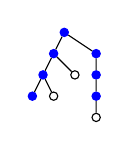
\begin{tikzpicture}[baseline=-0.5ex, scale=0.27]
    \tikzset{every node/.style={draw, circle, inner sep=0.5pt, minimum size=3pt}}
    \node[fill=Blue, draw=Blue] (NG) at (-1.80, -3) {};
    \node[] (NH) at (-0.80, -3) {};
    \node[fill=Blue, draw=Blue] (ND) at (-1.30, -2) {};
    \node[] (NE) at (0.20, -2) {};
    \node[fill=Blue, draw=Blue] (NB) at (-0.80, -1) {};
    \node[] (NJ) at (1.20, -4) {};
    \node[fill=Blue, draw=Blue] (NI) at (1.20, -3) {};
    \node[fill=Blue, draw=Blue] (NF) at (1.20, -2) {};
    \node[fill=Blue, draw=Blue] (NC) at (1.20, -1) {};
    \node[fill=Blue, draw=Blue] (NA) at (-0.30, 0) {};
    \draw (NA) -- (NB);
    \draw (NB) -- (ND);
    \draw (ND) -- (NG);
    \draw (ND) -- (NH);
    \draw (NB) -- (NE);
    \draw (NA) -- (NC);
    \draw (NC) -- (NF);
    \draw (NF) -- (NI);
    \draw (NI) -- (NJ);
  \end{tikzpicture}
}
\newsavebox{\boxshapeaq}
\sbox{\boxshapeaq}{
  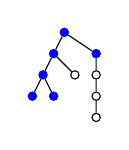
\begin{tikzpicture}[baseline=-0.5ex, scale=0.27]
    \tikzset{every node/.style={draw, circle, inner sep=0.5pt, minimum size=3pt}}
    \node[fill=Blue, draw=Blue] (NG) at (-1.80, -3) {};
    \node[fill=Blue, draw=Blue] (NH) at (-0.80, -3) {};
    \node[fill=Blue, draw=Blue] (ND) at (-1.30, -2) {};
    \node[] (NE) at (0.20, -2) {};
    \node[fill=Blue, draw=Blue] (NB) at (-0.80, -1) {};
    \node[] (NJ) at (1.20, -4) {};
    \node[] (NI) at (1.20, -3) {};
    \node[] (NF) at (1.20, -2) {};
    \node[fill=Blue, draw=Blue] (NC) at (1.20, -1) {};
    \node[fill=Blue, draw=Blue] (NA) at (-0.30, 0) {};
    \draw (NA) -- (NB);
    \draw (NB) -- (ND);
    \draw (ND) -- (NG);
    \draw (ND) -- (NH);
    \draw (NB) -- (NE);
    \draw (NA) -- (NC);
    \draw (NC) -- (NF);
    \draw (NF) -- (NI);
    \draw (NI) -- (NJ);
  \end{tikzpicture}
}
\newsavebox{\boxshapear}
\sbox{\boxshapear}{
  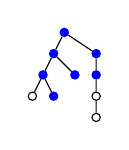
\begin{tikzpicture}[baseline=-0.5ex, scale=0.27]
    \tikzset{every node/.style={draw, circle, inner sep=0.5pt, minimum size=3pt}}
    \node[] (NG) at (-1.80, -3) {};
    \node[fill=Blue, draw=Blue] (NH) at (-0.80, -3) {};
    \node[fill=Blue, draw=Blue] (ND) at (-1.30, -2) {};
    \node[fill=Blue, draw=Blue] (NE) at (0.20, -2) {};
    \node[fill=Blue, draw=Blue] (NB) at (-0.80, -1) {};
    \node[] (NJ) at (1.20, -4) {};
    \node[] (NI) at (1.20, -3) {};
    \node[fill=Blue, draw=Blue] (NF) at (1.20, -2) {};
    \node[fill=Blue, draw=Blue] (NC) at (1.20, -1) {};
    \node[fill=Blue, draw=Blue] (NA) at (-0.30, 0) {};
    \draw (NA) -- (NB);
    \draw (NB) -- (ND);
    \draw (ND) -- (NG);
    \draw (ND) -- (NH);
    \draw (NB) -- (NE);
    \draw (NA) -- (NC);
    \draw (NC) -- (NF);
    \draw (NF) -- (NI);
    \draw (NI) -- (NJ);
  \end{tikzpicture}
}
\newsavebox{\boxshapeas}
\sbox{\boxshapeas}{
  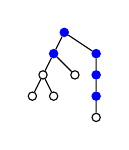
\begin{tikzpicture}[baseline=-0.5ex, scale=0.27]
    \tikzset{every node/.style={draw, circle, inner sep=0.5pt, minimum size=3pt}}
    \node[] (NG) at (-1.80, -3) {};
    \node[] (NH) at (-0.80, -3) {};
    \node[] (ND) at (-1.30, -2) {};
    \node[] (NE) at (0.20, -2) {};
    \node[fill=Blue, draw=Blue] (NB) at (-0.80, -1) {};
    \node[] (NJ) at (1.20, -4) {};
    \node[fill=Blue, draw=Blue] (NI) at (1.20, -3) {};
    \node[fill=Blue, draw=Blue] (NF) at (1.20, -2) {};
    \node[fill=Blue, draw=Blue] (NC) at (1.20, -1) {};
    \node[fill=Blue, draw=Blue] (NA) at (-0.30, 0) {};
    \draw (NA) -- (NB);
    \draw (NB) -- (ND);
    \draw (ND) -- (NG);
    \draw (ND) -- (NH);
    \draw (NB) -- (NE);
    \draw (NA) -- (NC);
    \draw (NC) -- (NF);
    \draw (NF) -- (NI);
    \draw (NI) -- (NJ);
  \end{tikzpicture}
}
\newsavebox{\boxshapeat}
\sbox{\boxshapeat}{
  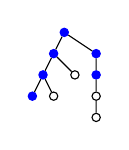
\begin{tikzpicture}[baseline=-0.5ex, scale=0.27]
    \tikzset{every node/.style={draw, circle, inner sep=0.5pt, minimum size=3pt}}
    \node[fill=Blue, draw=Blue] (NG) at (-1.80, -3) {};
    \node[] (NH) at (-0.80, -3) {};
    \node[fill=Blue, draw=Blue] (ND) at (-1.30, -2) {};
    \node[] (NE) at (0.20, -2) {};
    \node[fill=Blue, draw=Blue] (NB) at (-0.80, -1) {};
    \node[] (NJ) at (1.20, -4) {};
    \node[] (NI) at (1.20, -3) {};
    \node[fill=Blue, draw=Blue] (NF) at (1.20, -2) {};
    \node[fill=Blue, draw=Blue] (NC) at (1.20, -1) {};
    \node[fill=Blue, draw=Blue] (NA) at (-0.30, 0) {};
    \draw (NA) -- (NB);
    \draw (NB) -- (ND);
    \draw (ND) -- (NG);
    \draw (ND) -- (NH);
    \draw (NB) -- (NE);
    \draw (NA) -- (NC);
    \draw (NC) -- (NF);
    \draw (NF) -- (NI);
    \draw (NI) -- (NJ);
  \end{tikzpicture}
}
\newsavebox{\boxshapeau}
\sbox{\boxshapeau}{
  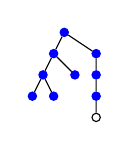
\begin{tikzpicture}[baseline=-0.5ex, scale=0.27]
    \tikzset{every node/.style={draw, circle, inner sep=0.5pt, minimum size=3pt}}
    \node[fill=Blue, draw=Blue] (NG) at (-1.80, -3) {};
    \node[fill=Blue, draw=Blue] (NH) at (-0.80, -3) {};
    \node[fill=Blue, draw=Blue] (ND) at (-1.30, -2) {};
    \node[fill=Blue, draw=Blue] (NE) at (0.20, -2) {};
    \node[fill=Blue, draw=Blue] (NB) at (-0.80, -1) {};
    \node[] (NJ) at (1.20, -4) {};
    \node[fill=Blue, draw=Blue] (NI) at (1.20, -3) {};
    \node[fill=Blue, draw=Blue] (NF) at (1.20, -2) {};
    \node[fill=Blue, draw=Blue] (NC) at (1.20, -1) {};
    \node[fill=Blue, draw=Blue] (NA) at (-0.30, 0) {};
    \draw (NA) -- (NB);
    \draw (NB) -- (ND);
    \draw (ND) -- (NG);
    \draw (ND) -- (NH);
    \draw (NB) -- (NE);
    \draw (NA) -- (NC);
    \draw (NC) -- (NF);
    \draw (NF) -- (NI);
    \draw (NI) -- (NJ);
  \end{tikzpicture}
}
\newsavebox{\boxshapeav}
\sbox{\boxshapeav}{
  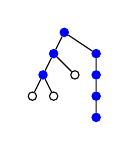
\begin{tikzpicture}[baseline=-0.5ex, scale=0.27]
    \tikzset{every node/.style={draw, circle, inner sep=0.5pt, minimum size=3pt}}
    \node[] (NG) at (-1.80, -3) {};
    \node[] (NH) at (-0.80, -3) {};
    \node[fill=Blue, draw=Blue] (ND) at (-1.30, -2) {};
    \node[] (NE) at (0.20, -2) {};
    \node[fill=Blue, draw=Blue] (NB) at (-0.80, -1) {};
    \node[fill=Blue, draw=Blue] (NJ) at (1.20, -4) {};
    \node[fill=Blue, draw=Blue] (NI) at (1.20, -3) {};
    \node[fill=Blue, draw=Blue] (NF) at (1.20, -2) {};
    \node[fill=Blue, draw=Blue] (NC) at (1.20, -1) {};
    \node[fill=Blue, draw=Blue] (NA) at (-0.30, 0) {};
    \draw (NA) -- (NB);
    \draw (NB) -- (ND);
    \draw (ND) -- (NG);
    \draw (ND) -- (NH);
    \draw (NB) -- (NE);
    \draw (NA) -- (NC);
    \draw (NC) -- (NF);
    \draw (NF) -- (NI);
    \draw (NI) -- (NJ);
  \end{tikzpicture}
}
\newsavebox{\boxshapeaw}
\sbox{\boxshapeaw}{
  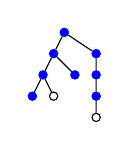
\begin{tikzpicture}[baseline=-0.5ex, scale=0.27]
    \tikzset{every node/.style={draw, circle, inner sep=0.5pt, minimum size=3pt}}
    \node[fill=Blue, draw=Blue] (NG) at (-1.80, -3) {};
    \node[] (NH) at (-0.80, -3) {};
    \node[fill=Blue, draw=Blue] (ND) at (-1.30, -2) {};
    \node[fill=Blue, draw=Blue] (NE) at (0.20, -2) {};
    \node[fill=Blue, draw=Blue] (NB) at (-0.80, -1) {};
    \node[] (NJ) at (1.20, -4) {};
    \node[fill=Blue, draw=Blue] (NI) at (1.20, -3) {};
    \node[fill=Blue, draw=Blue] (NF) at (1.20, -2) {};
    \node[fill=Blue, draw=Blue] (NC) at (1.20, -1) {};
    \node[fill=Blue, draw=Blue] (NA) at (-0.30, 0) {};
    \draw (NA) -- (NB);
    \draw (NB) -- (ND);
    \draw (ND) -- (NG);
    \draw (ND) -- (NH);
    \draw (NB) -- (NE);
    \draw (NA) -- (NC);
    \draw (NC) -- (NF);
    \draw (NF) -- (NI);
    \draw (NI) -- (NJ);
  \end{tikzpicture}
}
\newsavebox{\boxshapeax}
\sbox{\boxshapeax}{
  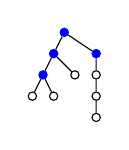
\begin{tikzpicture}[baseline=-0.5ex, scale=0.27]
    \tikzset{every node/.style={draw, circle, inner sep=0.5pt, minimum size=3pt}}
    \node[] (NG) at (-1.80, -3) {};
    \node[] (NH) at (-0.80, -3) {};
    \node[fill=Blue, draw=Blue] (ND) at (-1.30, -2) {};
    \node[] (NE) at (0.20, -2) {};
    \node[fill=Blue, draw=Blue] (NB) at (-0.80, -1) {};
    \node[] (NJ) at (1.20, -4) {};
    \node[] (NI) at (1.20, -3) {};
    \node[] (NF) at (1.20, -2) {};
    \node[fill=Blue, draw=Blue] (NC) at (1.20, -1) {};
    \node[fill=Blue, draw=Blue] (NA) at (-0.30, 0) {};
    \draw (NA) -- (NB);
    \draw (NB) -- (ND);
    \draw (ND) -- (NG);
    \draw (ND) -- (NH);
    \draw (NB) -- (NE);
    \draw (NA) -- (NC);
    \draw (NC) -- (NF);
    \draw (NF) -- (NI);
    \draw (NI) -- (NJ);
  \end{tikzpicture}
}
\newsavebox{\boxshapeay}
\sbox{\boxshapeay}{
  \begin{tikzpicture}[baseline=-0.5ex, scale=0.27]
    \tikzset{every node/.style={draw, circle, inner sep=0.5pt, minimum size=3pt}}
    \node[] (NG) at (-1.80, -3) {};
    \node[] (NH) at (-0.80, -3) {};
    \node[fill=Blue, draw=Blue] (ND) at (-1.30, -2) {};
    \node[] (NE) at (0.20, -2) {};
    \node[fill=Blue, draw=Blue] (NB) at (-0.80, -1) {};
    \node[] (NJ) at (1.20, -4) {};
    \node[] (NI) at (1.20, -3) {};
    \node[fill=Blue, draw=Blue] (NF) at (1.20, -2) {};
    \node[fill=Blue, draw=Blue] (NC) at (1.20, -1) {};
    \node[fill=Blue, draw=Blue] (NA) at (-0.30, 0) {};
    \draw (NA) -- (NB);
    \draw (NB) -- (ND);
    \draw (ND) -- (NG);
    \draw (ND) -- (NH);
    \draw (NB) -- (NE);
    \draw (NA) -- (NC);
    \draw (NC) -- (NF);
    \draw (NF) -- (NI);
    \draw (NI) -- (NJ);
  \end{tikzpicture}
}
\newsavebox{\boxshapeaz}
\sbox{\boxshapeaz}{
  \begin{tikzpicture}[baseline=-0.5ex, scale=0.27]
    \tikzset{every node/.style={draw, circle, inner sep=0.5pt, minimum size=3pt}}
    \node[] (NG) at (-1.80, -3) {};
    \node[fill=Blue, draw=Blue] (NH) at (-0.80, -3) {};
    \node[fill=Blue, draw=Blue] (ND) at (-1.30, -2) {};
    \node[] (NE) at (0.20, -2) {};
    \node[fill=Blue, draw=Blue] (NB) at (-0.80, -1) {};
    \node[fill=Blue, draw=Blue] (NJ) at (1.20, -4) {};
    \node[fill=Blue, draw=Blue] (NI) at (1.20, -3) {};
    \node[fill=Blue, draw=Blue] (NF) at (1.20, -2) {};
    \node[fill=Blue, draw=Blue] (NC) at (1.20, -1) {};
    \node[fill=Blue, draw=Blue] (NA) at (-0.30, 0) {};
    \draw (NA) -- (NB);
    \draw (NB) -- (ND);
    \draw (ND) -- (NG);
    \draw (ND) -- (NH);
    \draw (NB) -- (NE);
    \draw (NA) -- (NC);
    \draw (NC) -- (NF);
    \draw (NF) -- (NI);
    \draw (NI) -- (NJ);
  \end{tikzpicture}
}
\newsavebox{\boxshapeba}
\sbox{\boxshapeba}{
  \begin{tikzpicture}[baseline=-0.5ex, scale=0.27]
    \tikzset{every node/.style={draw, circle, inner sep=0.5pt, minimum size=3pt}}
    \node[fill=Blue, draw=Blue] (NG) at (-1.80, -3) {};
    \node[] (NH) at (-0.80, -3) {};
    \node[fill=Blue, draw=Blue] (ND) at (-1.30, -2) {};
    \node[fill=Blue, draw=Blue] (NE) at (0.20, -2) {};
    \node[fill=Blue, draw=Blue] (NB) at (-0.80, -1) {};
    \node[fill=Blue, draw=Blue] (NJ) at (1.20, -4) {};
    \node[fill=Blue, draw=Blue] (NI) at (1.20, -3) {};
    \node[fill=Blue, draw=Blue] (NF) at (1.20, -2) {};
    \node[fill=Blue, draw=Blue] (NC) at (1.20, -1) {};
    \node[fill=Blue, draw=Blue] (NA) at (-0.30, 0) {};
    \draw (NA) -- (NB);
    \draw (NB) -- (ND);
    \draw (ND) -- (NG);
    \draw (ND) -- (NH);
    \draw (NB) -- (NE);
    \draw (NA) -- (NC);
    \draw (NC) -- (NF);
    \draw (NF) -- (NI);
    \draw (NI) -- (NJ);
  \end{tikzpicture}
}
\newsavebox{\boxshapebb}
\sbox{\boxshapebb}{
  \begin{tikzpicture}[baseline=-0.5ex, scale=0.27]
    \tikzset{every node/.style={draw, circle, inner sep=0.5pt, minimum size=3pt}}
    \node[] (NG) at (-1.80, -3) {};
    \node[] (NH) at (-0.80, -3) {};
    \node[] (ND) at (-1.30, -2) {};
    \node[] (NE) at (0.20, -2) {};
    \node[fill=Blue, draw=Blue] (NB) at (-0.80, -1) {};
    \node[] (NJ) at (1.20, -4) {};
    \node[] (NI) at (1.20, -3) {};
    \node[] (NF) at (1.20, -2) {};
    \node[] (NC) at (1.20, -1) {};
    \node[fill=Blue, draw=Blue] (NA) at (-0.30, 0) {};
    \draw (NA) -- (NB);
    \draw (NB) -- (ND);
    \draw (ND) -- (NG);
    \draw (ND) -- (NH);
    \draw (NB) -- (NE);
    \draw (NA) -- (NC);
    \draw (NC) -- (NF);
    \draw (NF) -- (NI);
    \draw (NI) -- (NJ);
  \end{tikzpicture}
}
\newsavebox{\boxshapebc}
\sbox{\boxshapebc}{
  \begin{tikzpicture}[baseline=-0.5ex, scale=0.27]
    \tikzset{every node/.style={draw, circle, inner sep=0.5pt, minimum size=3pt}}
    \node[] (NG) at (-1.80, -3) {};
    \node[] (NH) at (-0.80, -3) {};
    \node[fill=Blue, draw=Blue] (ND) at (-1.30, -2) {};
    \node[fill=Blue, draw=Blue] (NE) at (0.20, -2) {};
    \node[fill=Blue, draw=Blue] (NB) at (-0.80, -1) {};
    \node[] (NJ) at (1.20, -4) {};
    \node[fill=Blue, draw=Blue] (NI) at (1.20, -3) {};
    \node[fill=Blue, draw=Blue] (NF) at (1.20, -2) {};
    \node[fill=Blue, draw=Blue] (NC) at (1.20, -1) {};
    \node[fill=Blue, draw=Blue] (NA) at (-0.30, 0) {};
    \draw (NA) -- (NB);
    \draw (NB) -- (ND);
    \draw (ND) -- (NG);
    \draw (ND) -- (NH);
    \draw (NB) -- (NE);
    \draw (NA) -- (NC);
    \draw (NC) -- (NF);
    \draw (NF) -- (NI);
    \draw (NI) -- (NJ);
  \end{tikzpicture}
}
\newsavebox{\boxshapebd}
\sbox{\boxshapebd}{
  \begin{tikzpicture}[baseline=-0.5ex, scale=0.27]
    \tikzset{every node/.style={draw, circle, inner sep=0.5pt, minimum size=3pt}}
    \node[] (NG) at (-1.80, -3) {};
    \node[] (NH) at (-0.80, -3) {};
    \node[] (ND) at (-1.30, -2) {};
    \node[] (NE) at (0.20, -2) {};
    \node[fill=Blue, draw=Blue] (NB) at (-0.80, -1) {};
    \node[fill=Blue, draw=Blue] (NJ) at (1.20, -4) {};
    \node[fill=Blue, draw=Blue] (NI) at (1.20, -3) {};
    \node[fill=Blue, draw=Blue] (NF) at (1.20, -2) {};
    \node[fill=Blue, draw=Blue] (NC) at (1.20, -1) {};
    \node[fill=Blue, draw=Blue] (NA) at (-0.30, 0) {};
    \draw (NA) -- (NB);
    \draw (NB) -- (ND);
    \draw (ND) -- (NG);
    \draw (ND) -- (NH);
    \draw (NB) -- (NE);
    \draw (NA) -- (NC);
    \draw (NC) -- (NF);
    \draw (NF) -- (NI);
    \draw (NI) -- (NJ);
  \end{tikzpicture}
}
\begin{tikzpicture}[scale=1.8]
\newcommand{\edgespathclr}{Blue}
\newcommand{\edgesclr}{gray}
\coordinate (A-B-D-E) at (4.00, 4);
\coordinate (A-B-C-D-G) at (7.11, 5);
\coordinate (A-B-C-D-F-G-H-I-J) at (5.33, 9);
\coordinate (A-B-E) at (5.33, 3);
\coordinate (A-B-C-D-F-H) at (3.56, 6);
\coordinate (empty) at (4.00, 0);
\coordinate (A-C-F-I) at (0.00, 4);
\coordinate (A-B-C-D-H) at (4.44, 5);
\coordinate (A-C-F-I-J) at (0.00, 5);
\coordinate (A-B-C-D-E) at (2.67, 5);
\coordinate (A-B-C-D-E-F-H-I) at (2.67, 8);
\coordinate (A-B-C-D-E-F-G-H-I-J) at (4.00, 10);
\coordinate (A-B-D-E-G) at (8.00, 5);
\coordinate (A-B-C-D-E-F) at (1.78, 6);
\coordinate (A-B-C-D-E-G-H) at (5.00, 7);
\coordinate (A-B-C) at (2.67, 3);
\coordinate (A-B-C-D-E-G) at (8.00, 6);
\coordinate (A-B-C-D-E-F-G) at (8.00, 7);
\coordinate (A-C-F) at (0.00, 3);
\coordinate (A-B-C-E) at (2.67, 4);
\coordinate (A-B-C-E-F) at (1.78, 5);
\coordinate (A-C) at (0.00, 2);
\coordinate (A-B-C-E-F-I-J) at (0.00, 7);
\coordinate (A-B-D-E-H) at (5.33, 5);
\coordinate (A-B-C-D-E-F-G-H) at (4.00, 8);
\coordinate (A) at (4.00, 1);
\coordinate (A-B-D-H) at (6.67, 4);
\coordinate (A-B-C-D-E-F-I-J) at (0.00, 8);
\coordinate (A-B-C-F) at (1.33, 4);
\coordinate (A-B-C-D-E-H) at (4.44, 6);
\coordinate (A-B-D-E-G-H) at (5.33, 6);
\coordinate (A-B-C-D-F-G-I-J) at (6.67, 8);
\coordinate (A-B-C-D-F-I) at (2.67, 6);
\coordinate (A-B-C-D-E-F-H-I-J) at (0.00, 9);
\coordinate (A-B-C-D-F-G-H) at (6.00, 7);
\coordinate (A-B-C-D-F-H-I) at (3.00, 7);
\coordinate (A-B-D-G) at (8.00, 4);
\coordinate (A-B-D) at (8.00, 3);
\coordinate (A-B-D-G-H) at (6.22, 5);
\coordinate (A-B-C-E-F-I) at (0.89, 6);
\coordinate (A-B-C-D-F-G-H-I) at (5.33, 8);
\coordinate (A-B-C-D-F-G-I) at (7.00, 7);
\coordinate (A-B-C-D-G-H) at (6.22, 6);
\coordinate (A-B-C-D-E-F-H) at (4.00, 7);
\coordinate (A-B-C-F-I) at (0.89, 5);
\coordinate (A-B-C-D-F-G) at (7.11, 6);
\coordinate (A-B-C-D-E-F-G-H-I) at (2.67, 9);
\coordinate (A-B-C-D-F-I-J) at (2.00, 7);
\coordinate (A-B-C-D-E-F-G-I) at (8.00, 8);
\coordinate (A-B-C-D) at (5.33, 4);
\coordinate (A-B-C-D-F) at (3.56, 5);
\coordinate (A-B-C-D-F-H-I-J) at (1.33, 8);
\coordinate (A-B-C-D-E-F-G-I-J) at (8.00, 9);
\coordinate (A-B) at (8.00, 2);
\coordinate (A-B-C-D-E-F-I) at (1.00, 7);
\coordinate (A-B-C-F-I-J) at (0.00, 6);
\foreach\a/\b in {
A-B-C-D-G/A-B-C-D-G-H, A-B-C-D-F-H/A-B-C-D-E-F-H, A-B-C-D-F-H-I/A-B-C-D-F-H-I-J, A-B-C-D-F-G-H-I-J/A-B-C-D-E-F-G-H-I-J, A-B-C-D-F-G-I/A-B-C-D-F-G-I-J, A-B-D-G-H/A-B-D-E-G-H, A-B-C-F/A-B-C-E-F, A-B-C-D-F-I/A-B-C-D-F-H-I, A-B-C-D-F-G-H-I/A-B-C-D-E-F-G-H-I, A-B-C-F-I/A-B-C-F-I-J, A-B-C-D-H/A-B-C-D-E-H, A-B-C-E/A-B-C-D-E, A-B-E/A-B-D-E, A-B-D-G/A-B-D-G-H, A/A-B, A-B-C-D-H/A-B-C-D-F-H, A-B-D-E-G-H/A-B-C-D-E-G-H, A-B-C-E-F-I/A-B-C-D-E-F-I, A-B-C-D-F-G/A-B-C-D-F-G-H, A-B-C-D-F-G-H/A-B-C-D-E-F-G-H, A-C-F-I/A-B-C-F-I, A-B-C/A-B-C-F, A-C/A-B-C, A-B-D-G/A-B-C-D-G, A-B-C-D-F-H-I-J/A-B-C-D-E-F-H-I-J, A-B-C/A-B-C-E, A-B-C-D/A-B-C-D-E, A-B-C-D-E/A-B-C-D-E-F, A-B-C-D-G/A-B-C-D-E-G, A-B-C-D-F-G-I/A-B-C-D-F-G-H-I, A-B-C-D-F/A-B-C-D-E-F, A-B-C-F-I-J/A-B-C-E-F-I-J, A-B-C-D-E-H/A-B-C-D-E-G-H, A-B-C-D-F-H/A-B-C-D-F-H-I, A-B-D-E/A-B-C-D-E, A-B-C-D-F-G/A-B-C-D-F-G-I, A-B-D/A-B-D-H, A-B-C-D-G/A-B-C-D-F-G, A-B-C-D/A-B-C-D-H, A-B-C-D-E-F-G-H/A-B-C-D-E-F-G-H-I, A-B-C-F/A-B-C-F-I, A-B-C-D-F-H-I/A-B-C-D-E-F-H-I, A-B-C-D-F-G/A-B-C-D-E-F-G, A-B-C-D-F-G-I/A-B-C-D-E-F-G-I, A-B-C-D-E-F-H/A-B-C-D-E-F-G-H, A-B-C-E-F/A-B-C-D-E-F, A-B-D/A-B-D-E, A-B-D-H/A-B-C-D-H, A-B-C-D-F-I-J/A-B-C-D-E-F-I-J, A-C-F/A-B-C-F, A-B-C-D-G-H/A-B-C-D-E-G-H, A-B-C-D-E-F-H-I/A-B-C-D-E-F-G-H-I, A-B-D-E-H/A-B-D-E-G-H, A-B/A-B-C, A-B-C-D-F-G-I-J/A-B-C-D-E-F-G-I-J, A-B-C-D-E-F/A-B-C-D-E-F-I, A-B-C-D-F/A-B-C-D-F-H, A-B-C-D-F-I/A-B-C-D-E-F-I, A-B-C-D-E-F-G-H-I/A-B-C-D-E-F-G-H-I-J, A-B-C-F-I/A-B-C-E-F-I, A-B-C-D-F-G-I-J/A-B-C-D-F-G-H-I-J, A-B-C-D-E-G-H/A-B-C-D-E-F-G-H, A-B-C-D-E-F-I/A-B-C-D-E-F-I-J}{
    \draw[\edgesclr] (\a) -- (\b);
}
\draw[\edgesclr] (A-B) -- (A-B-D);
\draw[\edgesclr] (A-B-D) -- (A-B-D-G);
\draw[\edgesclr] (A-B-C-D-E-F-I-J) -- (A-B-C-D-E-F-H-I-J);
\draw[\edgesclr] (A-B-C-D-E-F-G-H-I-J) -- (A-B-C-D-E-F-G-I-J);

\foreach\a/\b in {
A-B-D/A-B-C-D, empty/A, A-B-D-G-H/A-B-C-D-G-H, A-B/A-B-E, A-B-C-D-E-G-H/A-B-D-E-G-H, A-B-C-D-F-H/A-B-C-D-H, A-C-F-I-J/A-B-C-F-I-J, A-B-C-D-F-I-J/A-B-C-D-F-H-I-J, A-B-C-D-E-F-G-H/A-B-C-D-E-G-H, A-B-C-D-F-H-I-J/A-B-C-D-F-H-I, A-B-C-E-F/A-B-C-E-F-I, A-B-C-D-F-G-H-I-J/A-B-C-D-F-G-I-J, A-B-C-D-E-F-I-J/A-B-C-D-E-F-I, A-B-C-D-F-I/A-B-C-D-F-I-J, A-B-C-D-G-H/A-B-C-D-F-G-H, A-B-C-F/A-B-C, A-B-D-E-G/A-B-C-D-E-G, A-B-C-D-E-H/A-B-C-D-E-F-H, A-B-D-H/A-B-D-E-H, A-C-F-I/A-C-F-I-J, A-B-D-G/A-B-D-E-G, A-B-E/A-B-C-E, A-B-C-D-E-F/A-B-C-D-E, A-B-C-D-F-G-I-J/A-B-C-D-F-G-I, A-B-C-D-F-G-H/A-B-C-D-F-G-H-I, A-B-C-D-F-G-I/A-B-C-D-F-G, A-B-C-E-F-I-J/A-B-C-D-E-F-I-J, A-B-C-D-F-G/A-B-C-D-G, A-B-C-D-E-F-H/A-B-C-D-E-F-H-I, A-B-C-F-I-J/A-B-C-F-I, A-B-D-E-H/A-B-C-D-E-H, A-B-C-F-I/A-B-C-F, A-B-C-E/A-B-C-E-F, A-B-C-D-E/A-B-D-E, A-B-C-D-G/A-B-D-G, A-B-C-D-E-F-H-I-J/A-B-C-D-E-F-G-H-I-J, A-B-D-E/A-B-D, A-B-C-D/A-B-C-D-F, A-B-D-E-G-H/A-B-D-G-H, A-B-C-D-E-F-I/A-B-C-D-E-F, A-B-C-D-E-F-G-H-I-J/A-B-C-D-E-F-G-H-I, A-B-C-D-E-F-G-H-I/A-B-C-D-E-F-G-H, A-B-C-D-F-H-I/A-B-C-D-F-H, A-B-C-D-F-G-H-I/A-B-C-D-F-G-H-I-J, A-B-C-D-E-F-G-I/A-B-C-D-E-F-G-I-J, A/A-C, A-B-C-D-E-G/A-B-C-D-E-F-G, A-B-C-D-H/A-B-D-H, A-B-C/A-B, A-B-C-E-F-I/A-B-C-E-F-I-J, A-B-C-D-F/A-B-C-D-F-I, A-B-C-D-E-F-G/A-B-C-D-E-F-G-I, A-B-C-D-E-F-H-I/A-B-C-D-E-F-H-I-J, A-C/A-C-F, A-C-F/A-C-F-I}{
    \draw[\edgespathclr, ultra thick] (\a) -- (\b);
}
\node[draw, fill=white, inner sep=2pt, rounded corners=2pt] at (A-B-D-E) {\usebox{\boxshapea}};
\node[draw, fill=white, inner sep=2pt, rounded corners=2pt] at (A-B-C-D-G) {\usebox{\boxshapeb}};
\node[draw, fill=white, inner sep=2pt, rounded corners=2pt] at (A-B-C-D-F-G-H-I-J) {\usebox{\boxshapec}};
\node[draw, fill=white, inner sep=2pt, rounded corners=2pt] at (A-B-E) {\usebox{\boxshaped}};
\node[draw, fill=white, inner sep=2pt, rounded corners=2pt] at (A-B-C-D-F-H) {\usebox{\boxshapee}};
\node[draw, fill=white, inner sep=2pt, rounded corners=2pt] at (empty) {\usebox{\boxshapef}};
\node[draw, fill=white, inner sep=2pt, rounded corners=2pt] at (A-C-F-I) {\usebox{\boxshapeg}};
\node[draw, fill=white, inner sep=2pt, rounded corners=2pt] at (A-B-C-D-H) {\usebox{\boxshapeh}};
\node[draw, fill=white, inner sep=2pt, rounded corners=2pt] at (A-C-F-I-J) {\usebox{\boxshapei}};
\node[draw, fill=white, inner sep=2pt, rounded corners=2pt] at (A-B-C-D-E) {\usebox{\boxshapej}};
\node[draw, fill=white, inner sep=2pt, rounded corners=2pt] at (A-B-C-D-E-F-H-I) {\usebox{\boxshapek}};
\node[draw, fill=white, inner sep=2pt, rounded corners=2pt] at (A-B-C-D-E-F-G-H-I-J) {\usebox{\boxshapel}};
\node[draw, fill=white, inner sep=2pt, rounded corners=2pt] at (A-B-D-E-G) {\usebox{\boxshapem}};
\node[draw, fill=white, inner sep=2pt, rounded corners=2pt] at (A-B-C-D-E-F) {\usebox{\boxshapen}};
\node[draw, fill=white, inner sep=2pt, rounded corners=2pt] at (A-B-C-D-E-G-H) {\usebox{\boxshapeo}};
\node[draw, fill=white, inner sep=2pt, rounded corners=2pt] at (A-B-C) {\usebox{\boxshapep}};
\node[draw, fill=white, inner sep=2pt, rounded corners=2pt] at (A-B-C-D-E-G) {\usebox{\boxshapeq}};
\node[draw, fill=white, inner sep=2pt, rounded corners=2pt] at (A-B-C-D-E-F-G) {\usebox{\boxshaper}};
\node[draw, fill=white, inner sep=2pt, rounded corners=2pt] at (A-C-F) {\usebox{\boxshapes}};
\node[draw, fill=white, inner sep=2pt, rounded corners=2pt] at (A-B-C-E) {\usebox{\boxshapet}};
\node[draw, fill=white, inner sep=2pt, rounded corners=2pt] at (A-B-C-E-F) {\usebox{\boxshapeu}};
\node[draw, fill=white, inner sep=2pt, rounded corners=2pt] at (A-C) {\usebox{\boxshapev}};
\node[draw, fill=white, inner sep=2pt, rounded corners=2pt] at (A-B-C-E-F-I-J) {\usebox{\boxshapew}};
\node[draw, fill=white, inner sep=2pt, rounded corners=2pt] at (A-B-D-E-H) {\usebox{\boxshapex}};
\node[draw, fill=white, inner sep=2pt, rounded corners=2pt] at (A-B-C-D-E-F-G-H) {\usebox{\boxshapey}};
\node[draw, fill=white, inner sep=2pt, rounded corners=2pt] at (A) {\usebox{\boxshapez}};
\node[draw, fill=white, inner sep=2pt, rounded corners=2pt] at (A-B-D-H) {\usebox{\boxshapeaa}};
\node[draw, fill=white, inner sep=2pt, rounded corners=2pt] at (A-B-C-D-E-F-I-J) {\usebox{\boxshapeab}};
\node[draw, fill=white, inner sep=2pt, rounded corners=2pt] at (A-B-C-F) {\usebox{\boxshapeac}};
\node[draw, fill=white, inner sep=2pt, rounded corners=2pt] at (A-B-C-D-E-H) {\usebox{\boxshapead}};
\node[draw, fill=white, inner sep=2pt, rounded corners=2pt] at (A-B-D-E-G-H) {\usebox{\boxshapeae}};
\node[draw, fill=white, inner sep=2pt, rounded corners=2pt] at (A-B-C-D-F-G-I-J) {\usebox{\boxshapeaf}};
\node[draw, fill=white, inner sep=2pt, rounded corners=2pt] at (A-B-C-D-F-I) {\usebox{\boxshapeag}};
\node[draw, fill=white, inner sep=2pt, rounded corners=2pt] at (A-B-C-D-E-F-H-I-J) {\usebox{\boxshapeah}};
\node[draw, fill=white, inner sep=2pt, rounded corners=2pt] at (A-B-C-D-F-G-H) {\usebox{\boxshapeai}};
\node[draw, fill=white, inner sep=2pt, rounded corners=2pt] at (A-B-C-D-F-H-I) {\usebox{\boxshapeaj}};
\node[draw, fill=white, inner sep=2pt, rounded corners=2pt] at (A-B-D-G) {\usebox{\boxshapeak}};
\node[draw, fill=white, inner sep=2pt, rounded corners=2pt] at (A-B-D) {\usebox{\boxshapeal}};
\node[draw, fill=white, inner sep=2pt, rounded corners=2pt] at (A-B-D-G-H) {\usebox{\boxshapeam}};
\node[draw, fill=white, inner sep=2pt, rounded corners=2pt] at (A-B-C-E-F-I) {\usebox{\boxshapean}};
\node[draw, fill=white, inner sep=2pt, rounded corners=2pt] at (A-B-C-D-F-G-H-I) {\usebox{\boxshapeao}};
\node[draw, fill=white, inner sep=2pt, rounded corners=2pt] at (A-B-C-D-F-G-I) {\usebox{\boxshapeap}};
\node[draw, fill=white, inner sep=2pt, rounded corners=2pt] at (A-B-C-D-G-H) {\usebox{\boxshapeaq}};
\node[draw, fill=white, inner sep=2pt, rounded corners=2pt] at (A-B-C-D-E-F-H) {\usebox{\boxshapear}};
\node[draw, fill=white, inner sep=2pt, rounded corners=2pt] at (A-B-C-F-I) {\usebox{\boxshapeas}};
\node[draw, fill=white, inner sep=2pt, rounded corners=2pt] at (A-B-C-D-F-G) {\usebox{\boxshapeat}};
\node[draw, fill=white, inner sep=2pt, rounded corners=2pt] at (A-B-C-D-E-F-G-H-I) {\usebox{\boxshapeau}};
\node[draw, fill=white, inner sep=2pt, rounded corners=2pt] at (A-B-C-D-F-I-J) {\usebox{\boxshapeav}};
\node[draw, fill=white, inner sep=2pt, rounded corners=2pt] at (A-B-C-D-E-F-G-I) {\usebox{\boxshapeaw}};
\node[draw, fill=white, inner sep=2pt, rounded corners=2pt] at (A-B-C-D) {\usebox{\boxshapeax}};
\node[draw, fill=white, inner sep=2pt, rounded corners=2pt] at (A-B-C-D-F) {\usebox{\boxshapeay}};
\node[draw, fill=white, inner sep=2pt, rounded corners=2pt] at (A-B-C-D-F-H-I-J) {\usebox{\boxshapeaz}};
\node[draw, fill=white, inner sep=2pt, rounded corners=2pt] at (A-B-C-D-E-F-G-I-J) {\usebox{\boxshapeba}};
\node[draw, fill=white, inner sep=2pt, rounded corners=2pt] at (A-B) {\usebox{\boxshapebb}};
\node[draw, fill=white, inner sep=2pt, rounded corners=2pt] at (A-B-C-D-E-F-I) {\usebox{\boxshapebc}};
\node[draw, fill=white, inner sep=2pt, rounded corners=2pt] at (A-B-C-F-I-J) {\usebox{\boxshapebd}};
\end{tikzpicture}
